\documentclass[10pt]{article}

\usepackage[utf8]{inputenc}
\usepackage[spanish]{babel}
\usepackage{graphicx}
\usepackage{hyperref}
\usepackage{geometry}
\usepackage{subfigure}
% ------------------ FROM TEMPLATE ----------------------%
\usepackage[T1]{fontenc} % Output font encoding for international characters
\usepackage{mathpazo} % Palatino fon
% -------------------------------------------------------%

\def\titulo{Integración y validación del software del computador de a bordo
  del UPMSat-2}
\def\autor{David Herrero Sánchez}
\def\supervisor{Juan Zamorano Flores}
\def\fecha{27 de Abril de 2018}

\hypersetup{
  linkcolor=black,
  colorlinks=true,
  urlcolor=blue
}

\def \toplen{0.98 in}
\def \bottomlen{0.98 in}
\def \leftlen{1.18 in}
\def \rightlen{1.18 in}

\geometry{
	a4paper,
	left=\leftlen,
	right=\rightlen,
	top=\toplen,
	bottom=\bottomlen
}
\setlength{\parindent}{0pt}
% \addtolength{\leftmargin}{-0.5cm}
% \addtolength{\textwidth}{1cm}
% \setlength{\parskip}{-0.1cm}

\begin{document}
%----------------------------------------------------------------------------------------
%	TITLE PAGE
%----------------------------------------------------------------------------------------

\begin{titlepage} % Suppresses displaying the page number on the title page and the subsequent page counts as page 1
	\newcommand{\HRule}{\rule{\linewidth}{0.5mm}} % Defines a new command for horizontal lines, change thickness here
	
	\center % Centre everything on the page
	
	%------------------------------------------------
	%	Headings
	%------------------------------------------------
        \begin{figure}[h]
          
\includegraphics[height=2.5cm, width=3cm]{fig/upm.jpg}
          \hfill
          
\includegraphics[height=2.5cm, width=2.5cm]{fig/fi.jpeg}
        \end{figure}
        \vspace*{1cm}
	\textsc{\LARGE Escuela Técnica Superior de Ingenieros Informáticos\\[0.5cm]
        Universidad Politécnica de Madrid}\\[2cm] % Main heading such as the name of your university/college
	
	\textsc{\Large Trabajo final de grado}\\[0.5cm] % Major heading such as course name
	
	\textsc{\large Memoria de Seguimiento}\\[0.5cm] % Minor heading such as course title
	
	%------------------------------------------------
	%	Title
	%------------------------------------------------
	
	\HRule\\[0.4cm]
	
	{\huge\bfseries \titulo}\\[0.4cm] % Title of your document
	
	\HRule\\[1.5cm]
	
	%------------------------------------------------
	%	Author(s)
	%------------------------------------------------
	
	\begin{minipage}{0.4\textwidth}
		\begin{flushleft}
			\large
			\textit{Autor}\\
			\textsc{\autor} % Your name
		\end{flushleft}
	\end{minipage}
	~
	\begin{minipage}{0.4\textwidth}
		\begin{flushright}
			\large
			\textit{Supervisor}\\
			\textsc{\supervisor} % Supervisor's name
		\end{flushright}
	\end{minipage}
	
	% If you don't want a supervisor, uncomment the two lines below and comment the code above
	%{\large\textit{Author}}\\
	%John \textsc{Smith} % Your name
	
	%------------------------------------------------
	%	Date
	%------------------------------------------------
	
	\vfill\vfill\vfill % Position the date 3/4 down the remaining page
	
	{\large\fecha} % Date, change the \today to a set date if you want to be precise
	
	%------------------------------------------------
	%	Logo
	%------------------------------------------------
	
	%\vfill\vfill
	%\includegraphics[width=0.2\textwidth]{placeholder.jpg}\\[1cm] % Include a department/university logo - this will require the graphicx package
	 
	%----------------------------------------------------------------------------------------
	
	\vfill % Push the date up 1/4 of the remaining page
	
\end{titlepage}

%----------------------------------------------------------------------------------------


\section{Descripción general del trabajo}
Mi Trabajo Final de Grado (TFG) consiste en la integración y validación del
software del computador de a bordo (OBC\footnote{Computador de a bordo u
  \textit{On Board Computer} en inglés.}) del satélite UPMSat-2.\\

  Para llevar a cabo esta tarea es necesario estudiar y aprender en detalle cómo
  funcionan los distintos subsistemas que componen el OBC así como la estructura
  de su software para poder corregir y depurar los errores.\\

  Cabe destacar que en la situación actual en la que me encuentro no existe un
  documento de especificación de requisitos software (SRS\footnote{Siglas de
    \textit{Software Requirements Specification} en inglés.}) definitivo, por lo
  que al trabajo hay que añadirle las reuniones con los ingenieros aeronáuticos
  del IDR/UPM puesto que ellos son los \textit{clientes} del software del OBC.\\

  Para poder verificar que el software integrado cumple con la SRS será
  necesario establecer un conjunto de pruebas de sistema a través del envío
  de telecomandos (TCs\footnote{Abreviatura de \textit{telecomandos}.}) al OBC de manera que se pueda comprobar que éste
  responde correctamente a los mismos y que no surge ningún error software.

  Por ello, será necesario crear un \textit{framework} que facilite esta tarea.\\

  \subsection{Lista de objetivos}
  La lista de objetivos previstos es la siguiente:
  \begin{itemize}
  \item Estudiar y comprender los distintos subsistemas del OBC.
  \item Estudiar el diseño y organización del software del OBC.
  \item Aprendizaje de las herramientas con las que se trabajará.
  \item Estudio, revisión y comprensión de la SRS.
  \item Diseño de pruebas de sistema.
  \item Validación y verificación de los requisitos de la SRS.
  \item Depuración de errores encontrados.
  \item Integrar todo el software del OBC.
  \item Reunirse cada cierto tiempo con los clientes.
  \item Implementación de nuevos requisitos que puedan surgir o que hayan sido
    modificados.
  \end{itemize}

\section{Lista de tareas}
La lista de tareas en las que he decidido dividir el trabajo es la siguiente:
\begin{itemize}
\item Estudio de la documentación.
  \begin{itemize}
  \item Estudio en detalle de la funcionalidad de cada subsistema y la
    interacción entre los mismos.
  \item Análisis de la estructura del software del OBC y su diseño.
  \item Estudio y análisis de la SRS.
  \end{itemize}

\item Desarrollo del framework de pruebas.
  \begin{itemize}
  \item Diseñar o buscar una estructura para poder escribir los TCs en un
    fichero de texto.
  \item Escribir un programa que trate dicho fichero.
  \item Diseñar una aplicación gráfica que permita crear estos ficheros de
    forma fácil, intuitiva y cómoda.
  \end{itemize}

\item Integrar el software del OBC.

\item Probar que el software integrado cumple con la SRS.
  \begin{itemize}
  \item Creación de ficheros de pruebas con pruebas de caja negra.
  \item Creación de ficheros de pruebas con pruebas de caja blanca.
  \item Observación de la respuesta del OBC a los TCs recibidos.
  \item Registro de bugs y comportamientos anómalos con respecto a lo
    especificado.
  \end{itemize}

\item Reunión con los clientes.
  \begin{itemize}
  \item Mostrarles los avances conseguidos.
  \item Preguntarles sobre cómo actuar ante casos no previstos ni indicados
    en la SRS.
  \item Actualizar los resquisitos existentes y añadir nuevos requisitos.
  \end{itemize}

\item Llevar a cabo los cambios necesarios para cumplir con los cambios en la
  SRS.
  
\end{itemize}



\section{Diagrama de Gantt}
\begin{figure}[h]
  \hspace*{-3.75cm}%
  % 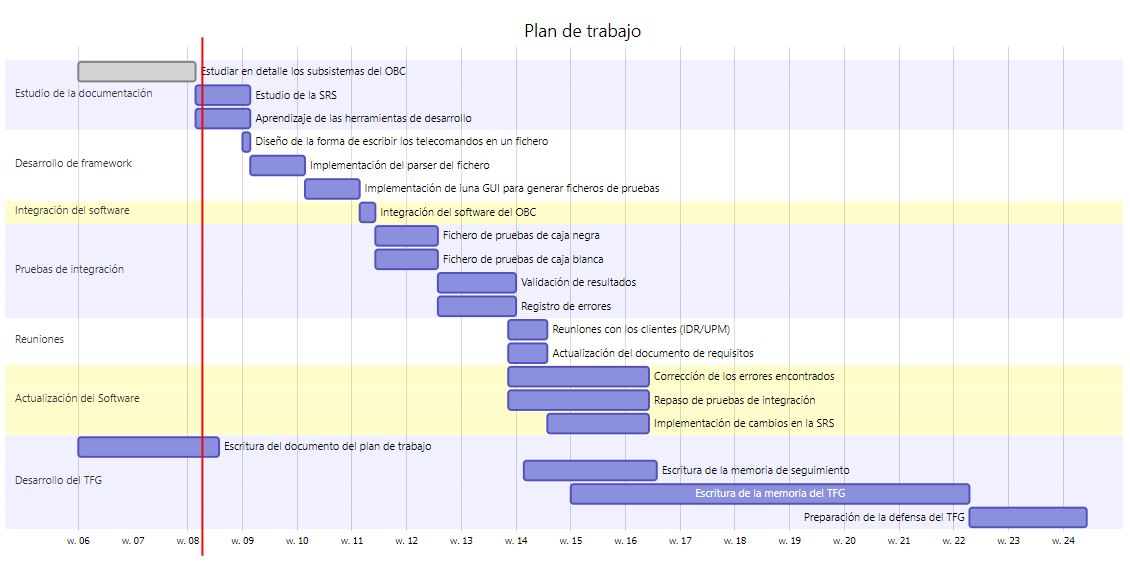
\includegraphics[width=1.5\textwidth]{fig/plan.JPG}
  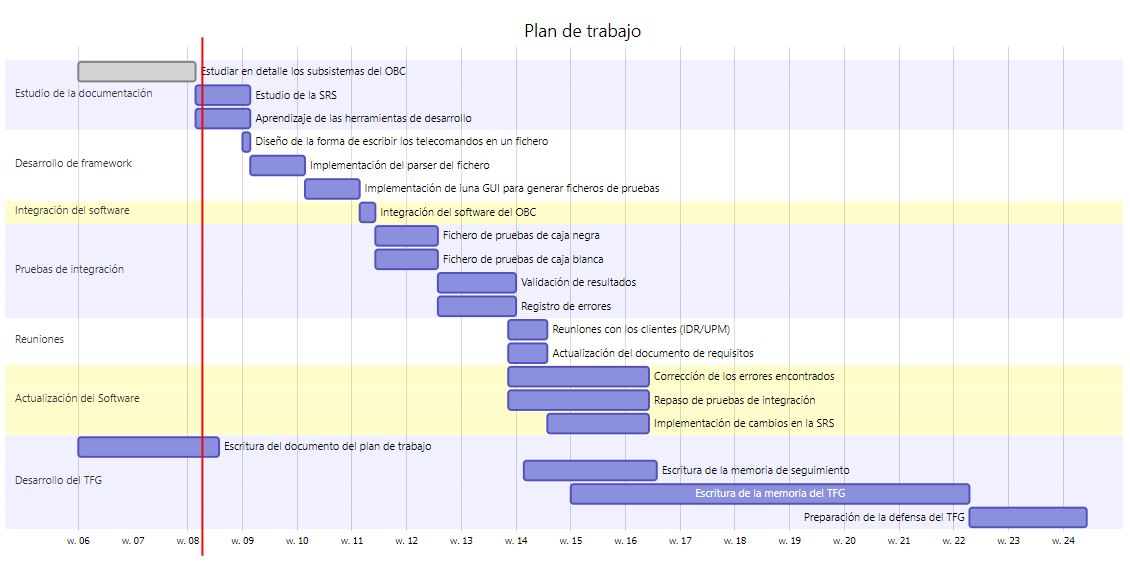
\includegraphics[scale=0.65]{fig/plan.JPG}
  \hspace*{-3.75cm}%
\end{figure}


\section{Borrador de la memoria final}
\label{sec:borrador}

En las siguientes páginas se adjunta el borrador de la memoria final del
TFG.
% 
\section{Propuesta de trabajo del tutor}

\paragraph{Título:}
Integración y validación del software del computador de a bordo del UPMSat-2.

\paragraph{Resumen del trabajo:}
UPMSat-2 es un proyecto de microsatélite universitario liderado por IDR/UPM y en
el que STRAST, nuestro grupo de investigación, se encarga del desarrollo del
software embarcado y del de la estación de tierra

(\url{http://www.idr.upm.es/tec\_espacial/upmsat2/01\_UPMSAT2.html}).

El trabajo consiste en la integración, pruebas de sistema y depuración de
errores de los distintos subsistemas que aportan la funcionalidad necesaria
para el correcto funcionamiento del segmento de vuelo.

Para ello se necesitan entrevistas con los ingenieros aeroespaciales a fin
de revisar el comportamiento final y el comportamiento ante fallos de hardware
y software.

\paragraph{Lista de objetivos concretos:}
\begin{itemize}
\item Estudio de los subsistemas y manejadores de dispositivos incluídos
  en el software.
\item Estudio del OBC (On-Board Computer) y de las herramientas de desarrollo,
  carga y depuración del software. Así como del sistema de validación
  del software.
\item Integración de todos estos subsistemas para generar el ejecutable
  del software.
\item Asignación de prioridades a las distintas tareas concurrentes para
  asegurar una ejecución correcta.
\item Desarrollo de un sistema de pruebas para pruebas de sistema.
\item Depuración de errores detectados y posibles desviaciones del
  comportamiento.
\item Desarrollo y adaptación de software a las nuevas necesidades.
\end{itemize}

\paragraph{Desglose de la dedicación total del trabajo en horas:}
\begin{itemize}
\item El alumno propuesto ha realizado el prácticum en el seno de este proyecto
  y posee conocimientos previos de desarrollo de software empotrado y tiempo
  real en el lenguaje de programación Ada.
\item No obstante, se estima en unas 100 horas la dedicación necesaria para
  aprender los requisitos del software de vuelo, sus distintos subsistemas y
  las herramientas necesarias para su integración y validación.
\item 50 horas para el desarrollo del sistema de pruebas que permita enviar
  órdenes y recibir telemetría del OBC de forma reproducible.
\item 65 horas de pruebas de integración, estudio de resultados e
  identificación de anomalías.
\item 60 horas para depurar los errores encontrados, entrevistas con
  el ``cliente'' (IDR/UPM) y realizar las modificaciones necesarias.
\item 49 horas para confeccionar la memoria y preparar la lectura.
\end{itemize}

\paragraph{Conocimientos prefios recomendados:}
Ingenería del software, programación y concurrencia, estructura de computadores,
sistemas empotrados, sistemas de tiempo real, entorno de desarrollo cruzado
de GNU sobre LinuX y lenguajes de programación Ada y C.

\end{document}
